\documentclass[
    12pt,				% tamanho da fonte
	openany,			% capítulos começam em qualquer tipo de pagina
	twoside,			% para impressão em recto e verso. Oposto a oneside
	a4paper,			% tamanho do papel.
	% -- opções da classe abntex2 --
	%chapter=TITLE,		% títulos de capítulos convertidos em letras maiúsculas
	%section=TITLE,		% títulos de seções convertidos em letras maiúsculas
	%subsection=TITLE,	% títulos de subseções convertidos em letras maiúsculas
	%subsubsection=TITLE,% títulos de subsubseções convertidos em letras maiúsculas
	% -- opções do pacote babel --
	english,			% idioma adicional para hifenização
	%french,				% idioma adicional para hifenização
	%spanish,			% idioma adicional para hifenização
	brazil, 			% o último idioma é o principal do documento
]{abntex2}

% ---
% PACOTES
% ---

% ---
% Pacotes Fundamentais
%---
\usepackage{lmodern}			% Usa a fonte Latin Modern
\usepackage[T1]{fontenc}		% Selecao de codigos de fonte.
\usepackage[utf8]{inputenc}		% Codificacao do documento (conversão automática dos acentos)
\usepackage{indentfirst}		% Indenta o primeiro parágrafo de cada seção.
\usepackage{color}				% Controle das cores
\usepackage{graphicx}			% Inclusão de gráficos
\usepackage{microtype} 			% para melhorias de justificação
\graphicspath{ {imagens/} }
% ---
% Pacotes de citações
% ---
\usepackage[brazilian,hyperpageref]{backref}	 % Paginas com as citações na bibl
\usepackage[alf]{abntex2cite}	                 % Citações padrão ABNT


\newcommand{\wiot}{\emph{IoT}}
% ---
% CONFIGURAÇÕES DE PACOTES
% ---
% ---
% Configurações do pacote backref
% Usado sem a opção hyperpageref de backref
\renewcommand{\backrefpagesname}{Citado na(s) página(s):~}
% Texto padrão antes do número das páginas
\renewcommand{\backref}{}
% Define os textos da citação
\renewcommand*{\backrefalt}[4]{
	\ifcase #1 %
		Nenhuma citação no texto.%
	\or
		Citado na página #2.%
	\else
		Citado #1 vezes nas páginas #2.%
	\fi}%
% ---

% ---
% Informações de dados para CAPA e FOLHA DE ROSTO
% ---
\titulo{Hedwig - Casa Automatizada}
\autor{
        Daniela Sayuri Yassuda \\
        Gabriela Souza de Melo   \\
        Hugo da Silva Possani    \\
        Victor Takashi Hayashi
}
\local{São Paulo}
\data{2017}
\instituicao{%
  Universidade de São Paulo -- USP
  \par
  Escola Politécnica
  \par
  Engenharia Elétrica -- Ênfase em Computação}
\tipotrabalho{Tese (Doutorado)}
% O preambulo deve conter o tipo do trabalho, o objetivo,
% o nome da instituição e a área de concentração
\preambulo{Modelo canônico de Projeto de pesquisa em conformidade
com as normas ABNT apresentado à comunidade de usuários \LaTeX.}
% ---

% ---
% Configurações de aparência do PDF final

% alterando o aspecto da cor azul
\definecolor{blue}{RGB}{41,5,195}

% informações do PDF
\makeatletter
\hypersetup{
     	%pagebackref=true,
		pdftitle={\@title},
		pdfauthor={\@author},
    	pdfsubject={\imprimirpreambulo},
	    pdfcreator={LaTeX with abnTeX2},
		pdfkeywords={abnt}{latex}{abntex}{abntex2}{projeto de pesquisa},
		colorlinks=true,       		% false: boxed links; true: colored links
    	linkcolor=blue,          	% color of internal links
    	citecolor=blue,        		% color of links to bibliography
    	filecolor=magenta,      	% color of file links
		urlcolor=blue,
		bookmarksdepth=4
}
\makeatother
% ---

% ---
% Espaçamentos entre linhas e parágrafos
% ---

% O tamanho do parágrafo é dado por:
\setlength{\parindent}{1.3cm}

% Controle do espaçamento entre um parágrafo e outro:
\setlength{\parskip}{0.2cm}  % tente também \onelineskip

% ---
% compila o indice
% ---
\makeindex
% ---

% ----
% Início do documento
% ----
\begin{document}

% Seleciona o idioma do documento (conforme pacotes do babel)
%\selectlanguage{english}
\selectlanguage{brazil}

% Retira espaço extra obsoleto entre as frases.
\frenchspacing

% ----------------------------------------------------------
% ELEMENTOS PRÉ-TEXTUAIS
% ----------------------------------------------------------
% \pretextual

% ---
% Capa
% ---
\imprimircapa
% ---

% ---
% inserir o sumario
% ---
\pdfbookmark[0]{\contentsname}{toc}
\tableofcontents*
\cleardoublepage
% ---

% ----------------------------------------------------------
% ELEMENTOS TEXTUAIS
% ----------------------------------------------------------
\textual

% ----------------------------------------------------------
% Introdução
% ----------------------------------------------------------
\chapter{Introdução}

O projeto Hedwig, trabalho de conclusão de curso do grupo, tem como objetivo aplicar os conceitos de \emph{Internet of Things} (IoT) para criar um sistema de automação residencial robusto e modularizado. Assim, o foco deste relatório está em analisar os aspectos desse projeto sob a ótica dos Sistemas de Informação (SI), que são o objeto de estudo da disciplina.

A temática do projeto fornece amplo material para que possam ser discutidos as diversas questões relacionadas aos Sistemas de Informação, visto que há o desenvolvimento de plataformas de hardware e software, a utilização de banco de dados e o seu uso envolve diversas questões atuais de segurança, ética e privacidade.

O projeto desenvolvido e apresentado pode ser viabilizado em produtos que poderiam expandir o mercado brasileiro de sistemas para casas inteligentes, de modo que a análise do ponto de vista empresarial oferece ganhos ao entendimento do trabalho, enriquecendo-o.

% TODO usar os números e porcentagens da introdução da monografia aqui?

\chapter{Breve Descrição do Projeto de Formatura}

O projeto de formatura tem como objetivo o desenvolvimento de um sistema de automação residencial completo, com foco na robustez, segurança e facilidade de uso. Para tanto, a modelagem de uma arquitetura flexível, mas que suportasse os requisitos iniciais, tem papel essencial no trabalho. A plataforma do sistema é enfática em sua proposta de camadas, na qual a integração entre os níveis é feito por meio de troca de mensagens, utilizando a infraestrutura de comunicação desenvolvida. No decorrer desta seção, serão apresentados os pontos essenciais do projeto, bem como a descrição das soluções adotadas.

\section{Hardware}

% TODO cada tipo de módulo
% TODO colocar fotos

\section{Software}

As partes de software do sistema são divididas de acordo com a sua aplicação, localização e uso. Neste momento, serão considerados somente os softwares de aplicação, de maneira que todo o software de operação do hardware está descrito na no item (MARCAR ITEM).

Em contato mais próximo dos dispositivos de hardware está o servidor local, Morpheus. O servidor local é responsável pela interconexão dos módulos da casa com os serviços de nuvem disponíveis. A troca de informação entre os módulos físicos e o Morpheus é realizada por meio de mensagens, codificadas em um protocolo desenvolvido pelo grupo, e encaminhadas por meio do protocolo MQTT, com um broker local disponível na residência. O envio de mensagens é feito em tópicos, aos quais o módulo pode publicar ou se inscrever de acordo com o seu serial number, de modo a evitar que um módulo consiga ter acesso ao canal de outro módulo. O servidor local, no entanto, precisa de um certificado válido para que possa se inscrever no seu canal, onde a troca de mensagens é realizada com criptografia assíncrona. Quando a mensagem chega nesse servidor, ela é convertida em um formato intermediário e colocada em um fila de entrada, onde uma thread de um pool irá retirá-la para efetuar o processamento, e conversão para um JSON esperado pela nuvem.

A segunda transmissão de dados, entre o Morpheus e os serviços de nuvem é feita por meio de um canal WebSocket, no qual a conexão permanece ativa a todo o momento. Os serviços de nuvem tratam a chegada da mensagem, e interagem com um cliente web, por meio de um dashboard, sobre o qual o usuário pode interagir.

% TODO imagens da dashboard

Para que a robustez do sistema seja assegurada, o projeto também conta com um sistema emergencial, no caso de não haver internet na casa ou de ocorrer qualquer problema com o servidor local. O usuário pode se conectar diretamente na rede de um dos módulos, sem a integração com a nuvem.

\section{Bases de Dados}

São usadas duas bases de dados na implementação do Hedwig. O primeiro é um banco de dados não-relacional baseado em documentos, que armazena dados coletados pelos sensores e informações sobre as entidades relevantes ao sistema - usuários e seus dispositivos conectados. O segundo é um banco de dados em memória que guarda informações sobre os dispositivos que estão conectados à nuvem no momento, facilitando a comunicação entre aplicativos e os controladores de cada casa.

% TODO imagem da arquitetura da nuvem

\subsection{Dados de Sensores, Dispositivos e Usuários}

É usado o MongoDB como banco de dados principal. O MongoDB é um banco de dados não-relacional, gratuito e \emph{open-source} baseado em documentos, que são representados como objetos com pares chave-valor similares aos objetos JSON. Essa escolha deve-se ao fato de que o maior volume de dados armazenados são os valores dos sensores, que podem ser facilmente modelados como documentos. Outros fatores que influenciaram a escolha do MongoDB foram sua escalabilidade, que pode ser realizada por replicação ou "clustering", e a flexibilidade de poder implementar facilmente mudanças nas propriedades das entidades.

\subsection{Dados de Conexões Ativas}

Para facilitar o encaminhamento de dados --- tanto informações coletadas pelos sensores como comandos de ação e configuração --- entre controladores locais e aplicativos cliente, foi usado o Redis, um banco de dados em memória capaz de armazenar estruturas como strings, listas, hashes, conjuntos ordenados e não-ordenados, indíces de geolocalização, entre outros. Devido à sua performance, o Redis é frequentemente usado para cache de páginas, aplicações de mensageria, implementação de filas e armazenamento de dados de sessão. No caso do Hedwig, ele é usado para esta última aplicação, guardando dados dos controladores e aplicativos conectados à nuvem no momento.

\section{Redes e Conectividade}

A conectividade local, planejada sobre a infraestrutura de comunicação disponível, é feita por meio de ondas de rádio, na frequência comercial relativa às redes Wi-Fi. Cada um dos módulos possui um microcontrolador e radiotransmissor ESP8266, o qual se conecta à rede da residência e envia mensagens para o respectivo tópico. Os módulos possuem tópicos específicos, cujos nomes são finalizados em "m2s" (\emph{module to server}) e contêm o serial ID do módulo em questão. Essa garantia é feita por meio de configurações no broker, no qual assegura-se dr que o endereço do tópico possui as credenciais do módulo autenticado.

O servidor local possui um tópico específico, cujo nome é finalizado em "s2m" (\emph{server to module}), e tem acesso de subscrição a todos os tópicos relativos às publicações de módulos. A autenticação do servidor, ao contrário daquela dos módulos, é feito por meio de certificados digitais, e há criptografia assíncrona na camada de transporte (SSL).

Para a comunicação entre a casa e a nuvem, ocorreram mudanças durante o planejamento da arquitetura. De início, o projeto estabelecia que o servidor local também tivesse a responsabilidade de ser um servidor para requisições externas, oferecendo para isso uma API REST. Entretanto, os impactos dessa decisão afetam criticamente a segurança, já que a casa estaria suscetível a ataques de negação de serviço (DoS). Assim, posteriormente, optou-se pela utilização de WebSockets na implementação dessa comunicação, de modo que a conexão entre controlador local e nuvem permanece ativa, e a responsabilidade por se proteger de ataque do tipo concentra-se nesta última, onde há uma infraestrutura muito mais robusta e existe possibilidade de uso de serviços de terceiros, como servidores Akamai.

Em alto nível, é representado na \autoref{fig:arquiteturaHedwig} o diagrama arquitetural do projeto. Na \autoref{fig:diagramaDeComunicacao}, é disponibilizada a arquitetura do servidor local (Morpheus) e a sua conectividade com a nuvem e módulos.

\begin{figure}[htb]
	\caption{\label{fig:arquiteturaHedwig}Diagrama Arquitetural}
	\begin{center}
	    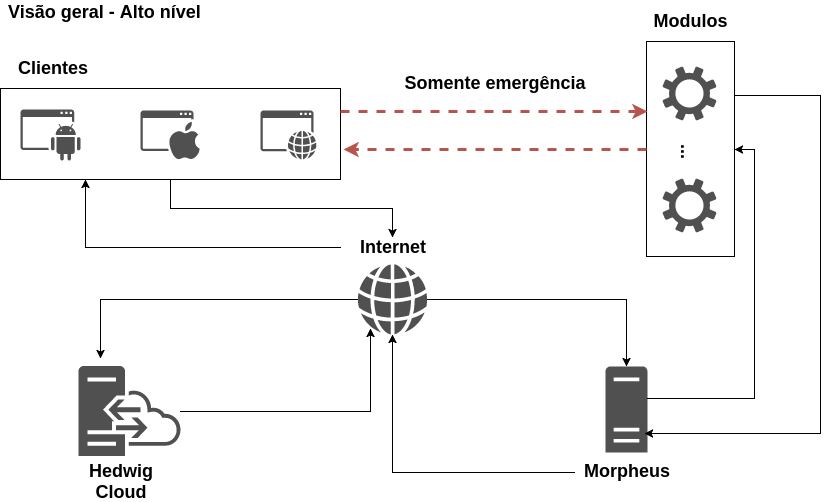
\includegraphics[scale=0.5]{arquiteturaHedwig}
	\end{center}
	\legend{Fonte: os autores}
\end{figure}

\begin{figure}[htb]
	\caption{\label{fig:diagramaDeComunicacao}Diagrama de Comunicação}
	\begin{center}
	    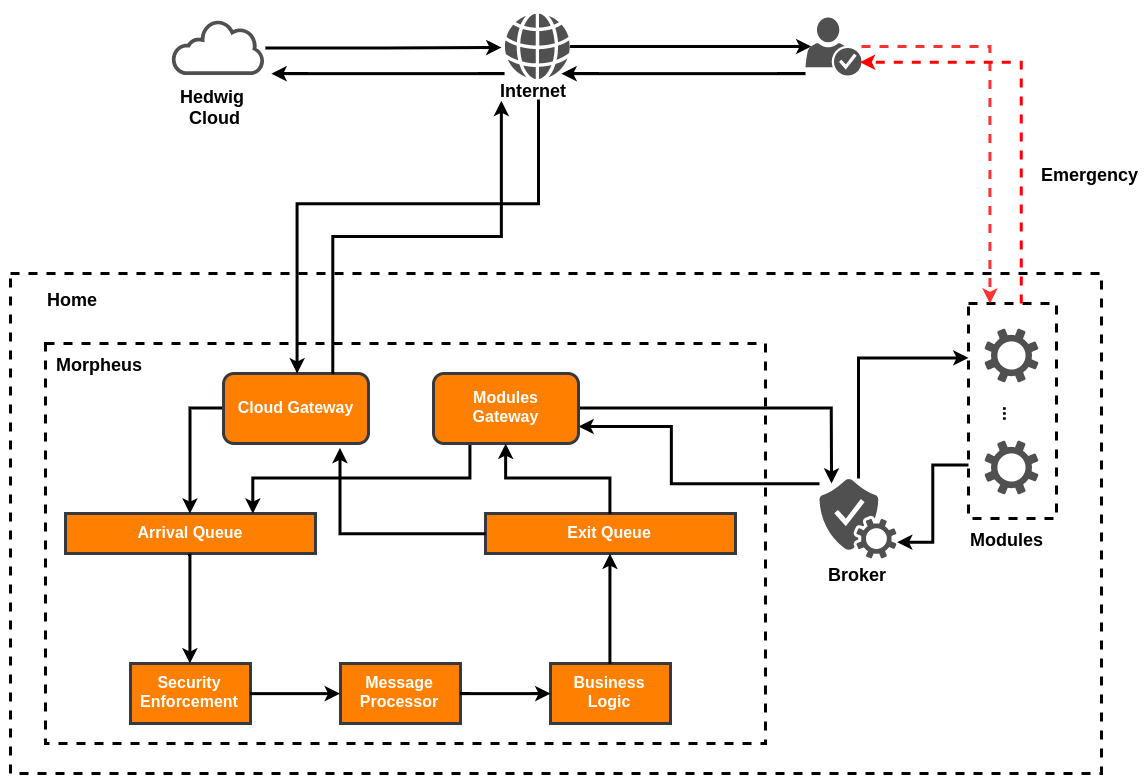
\includegraphics[scale=0.4]{diagramaDeComunicacao}
	\end{center}
	\legend{Fonte: os autores}
\end{figure}

% TODO diagrama de interação

\chapter{Características de SI}

\section{Aspectos Tecnológicos, Organizacionais e de Pessoas}

Para uma análise completa das características do Sistema de Informação, faz-se necessário o entendimento de suas três dimensões essenciais: organização, pessoas e tecnologia. O projeto desenvolvido é uma relevante contribuição às tecnologias de IoT e promove uma alternativa de baixo custo, adaptada à realidade e ao mercado nacional.

\subsection{Tecnologia}

Do ponto de vista tecnológico, o sistema busca a automação residencial, com a qual o usuário pode ter acesso à sua casa remotamente por meio da operação de um cliente web, com mobilidade, segurança e facilidade de uso. Foram desenvolvidos módulos físicos, cuja implementação tem seu núcleo no componente ESP8266, módulo com capacidade de processamento e radiotransmissão adequada aos padrões IEEE 802.11 -- WiFi. Por meio de transdutores e atuadores, acoplados aos módulos, o sistema obtém dados sobre o estado atual da casa (temperatura, umidade, luminosidade, etc) e pode agir sobre outros componentes (como o acendimento de uma lâmpada, ou a abertura dos portões). A comunicação entre os módulos e os serviços de nuvens passa pelo servidor local, que se conectará diretamente aos servidores remotos por meio de um canal seguro e protegido.

O uso de tecnologias modernas nas plataformas criadas é natural ao usuário, de modo que o seu emprego é transparente, e garante familiaridade e facilidade quando operada. Assim, o cliente não necessita da compra de algum outro dispositivo específico para interagir com sua casa. O seu smartphone, que já é utilizado no dia a dia, entra como o principal mecanismo de controle e troca de informações com a casa inteligente. A criação de uma dashboard responsiva, permite que o painel de controle da casa possa ser acessado tanto por computadores pessoais (PCs) quanto por tablets e smartphones, sem que a experiência do usuário (UX - User Experience) seja afetada pela troca.

% TODO falar mais do aplicativo cliente do ponto de vista tecnológico

\subsection{Organização}

Do ponto de vista organizacional, a empresa criada (Hedwig) estará continuamente buscando uma relação mais próxima a seus clientes. O conhecimento obtido a partir da análise de dados das casas é utilizado para a melhoria dos sistemas existentes, de modo que possam ser adaptados às necessidades e padrões de uso do morador. Utilizando-se técnicas de \emph{Business Intelligence} podem-se desenvolver novos produtos para suprir demandas específicas, que passarão a ser conhecidas. Um dos maiores desafios organizacionais para a empresa é a segurança dos dados obtidos, bem como da interação entre a casa e o cliente. Um possível ataque poderia sequestrar informações confidenciais ou roubar o acesso do cliente à casa, podendo trazer danos irreparáveis tanto aos nossos usuários quanto à Hedwig, que perderá a confiança e o prestígio.

\subsection{Pessoas}

Na dimensão de pessoas, o projeto realiza uma quebra de paradigma com a realidade atual dos nossos usuários. Sua casa começaria a ser vista como um local inteligente, integrado com sua rotina, e que pode entender os seus padrões, gostos e preferências. A ruptura promovida justamente faz frente à histórica visão da casa como simplesmente o seu refúgio diário, de proteção e descanso. Quando fora, não é possível controle ou observação de estado, do que acontece dentro, e quando dentro, tudo que se deseja é feito por meio da interação física com o que se deseja.

Assim, há uma mudança nos costumes de cada um, o que inicialmente traz resistência natural, mas que deve ser trabalhada para que o sistema se torne tão espontâneo quanto o antigo conceito. A resistência encontrada é, primordialmente, no que diz respeito à segurança. Com todas as cyber ameaças, apresentadas diariamente nos meios de comunicação, o medo de que a sua casa seja tomada por pessoas mal intencionadas se faz presente. Além disso, também há preocupações nos casos de falha, mesmo as que fogem do controle do projeto, como a interrupção no fornecimento de energia elétrica.

Tais desafios devem ser observados e atendidos pelo sistema, de modo que não haja conflito com o usuário, mas trabalho em conjunto para que o todo seja continuamente melhorado, com base nas percepções do cliente e na análise dos dados obtidos.

\section{Produção, RH, Finanças/Contabilidade e Vendas/Marketing}

\subsection{Produção}

Desde o início, o baixo custo de produção na elaboração do projeto foi uma das prioridades. O baixo custo é determinante porque, com base na realidade nacional, as perspectivas de expansão só podem ser concretizadas se houver viabilidade para a implementação no maior número possível de residências. Assim, levando-se em conta que a automação de sua casa não é uma prioridade para a maioria das famílias no Brasil, cuja renda é significativamente inferior à renda média de países desenvolvidos, um produto caro, desta natureza, mesmo que ofereça melhores acabamentos, não terá condições de ser adquirido por um número alto de consumidores fora dos grandes centros.

Os módulos projetados são pequenos e simples de serem desenvolvidos em escala. A parte mais essencial é o componente ESP8266, conforme explicado anteriormente. Assim, é necessário o contato diretamente com empresas fornecedoras, com o estabelecimento de contratos cujos valores unitários sejam baixos para quantidades elevadas.

Os sistemas de software serão desenvolvidos por uma equipe altamente qualificada e, posteriormente aos testes, distribuídos aos usuários em formas de atualizações. Tais atualizações podem ser gratuitas, para correções ou mudanças que afetam a segurança ou performance, ou pagas, quando há a inserção de novas funcionalidades.

Planeja-se a utilização de softwares de gestão da cadeia de suprimento para o controle e otimização da produção, por meio de um modelo Pull.

\subsection{Recursos Humanos}

O departamento de recursos humanos da empresa (RH) será responsável por atrair novos talentos alinhados à cultura e às propostas da empresa, bem como na manutenção dos funcionários presentes. O desenvolvimento de uma cultura interna na empresa é essencial para manter os funcionários sempre extremamente motivados e alavancando cada vez mais a empresa. 

Serão utilizadas ferramentas de Gestão de Relacionamento com o Funcionário (ERM), para que haja maior contato e feedback entre os colaboradores.

\subsection{Finanças e Contabilidade}

O departamento de finanças e contabilidade serão responsáveis por toda a organização fiscal da empresa, bem como pela geração dos relatórios de vendas, custos, compras de matéria prima, etc. Assim como o departamento de Recursos Humanos, os departamentos de finanças e contabilidade farão uso de Aplicações Integradas, fornecidas por empresas responsáveis e de tradição na área.

\subsection{Vendas e Marketing}

Todo o processo de venda será analisado internamente, para que possam ser obtidos dados do negócio, bem como um entendimento amplo sobre quem são nossos clientes, quais as suas expectativas, e as motivações para a escolha do produto. Principalmente em termos de marketing, serão buscados acordos com lojas que vendem materiais para construção, frequentadas por pessoas que estão reformando suas residências e sempre buscam por alguma inovação ou melhoria para sua casa.

Como se trata de um produto novo, ainda não conhecido por grande parte da população, é necessário que também sejam realizadas propagandas, para que haja uma popularização dos conceitos trazidos, bem como para a demonstração das vantagens que a plataforma oferece.

\section{Cadeia de Suprimento, Forças Competitivas e Cadeia de Valor}

\subsection{Cadeia de Suprimento}

A matéria-prima necessária ao desenvolvimento dos módulos constitui-se, majoritariamente, de componentes eletrônicos, como resistores, capacitores, relés, e outros produtos mais elaborados, como sensores de luminosidade, temperatura e umidade, atuadores diversos, microcontroladores  e radiotransmissores. Os maiores produtores mundiais desses produtos estão localizados na China, mas possuem uma ampla e bem estabelecida rede de transporte para o Brasil.

A instalação inicial da fábrica será no Estado de São Paulo, para onde a matéria prima será transportada, por via terrestre, em caminhões. Serão realizados contratos e acordos diversos, para que os preços sejam negociados, bem como os planejamentos para abastecimento do estoque de material. Assim, um número reduzido e otimizado de fretamentos pode suprir as necessidades, de modo que os custos sejam reduzidos.

As placas de fenolite, com o circuito impresso, serão projetadas e enviadas para produção na China, também a um custo reduzido. A qualidade do produto é muito mais elevada, quando elaborado em uma fábrica que possui equipamentos de usinagem modernos, e alguns componentes essenciais podem ser soldados na própria instalação.

Os controladores serão gravados com a versão atualizada do firmware e, após isso, será também soldado na placa, sendo este um dos últimos passos do processo de montagem física. Após isso, devem ser realizados testes padrões e automatizados, para garantir que os módulos estejam funcionando normalmente.

O estoque deve ser mínimo, de modo a manter os custos e gastos o mais baixo possível. Por isso a necessidade de boas técnicas de \emph{Business Intelligence}, para que sejam estudados os comportamentos de demanda e uso do produto, e para que essa demanda seja atendida sempre que necessário.

Para o transporte, deverá ser realizado um estudo inicial de logística, analisando as rotas mais viáveis e econômicas para levar o produto até os compradores. Para vendas pequenas, pode-se utilizar serviços já disponíveis no mercado, e para vendas maiores, uma empresa de fretamento poderá ser contratada.

\subsection{Forças Competitivas}

Na \autoref{fig:porter}, é possível visualizar as cincos forças competitivas de Porter, de modo que seja analisado o negócio, mas pelo lado externo, para que obtenção de sua atratividade e valor.

\begin{figure}[H]
	\caption{\label{fig:porter}Cinco forças competitivas de Porter}
	\begin{center}
	    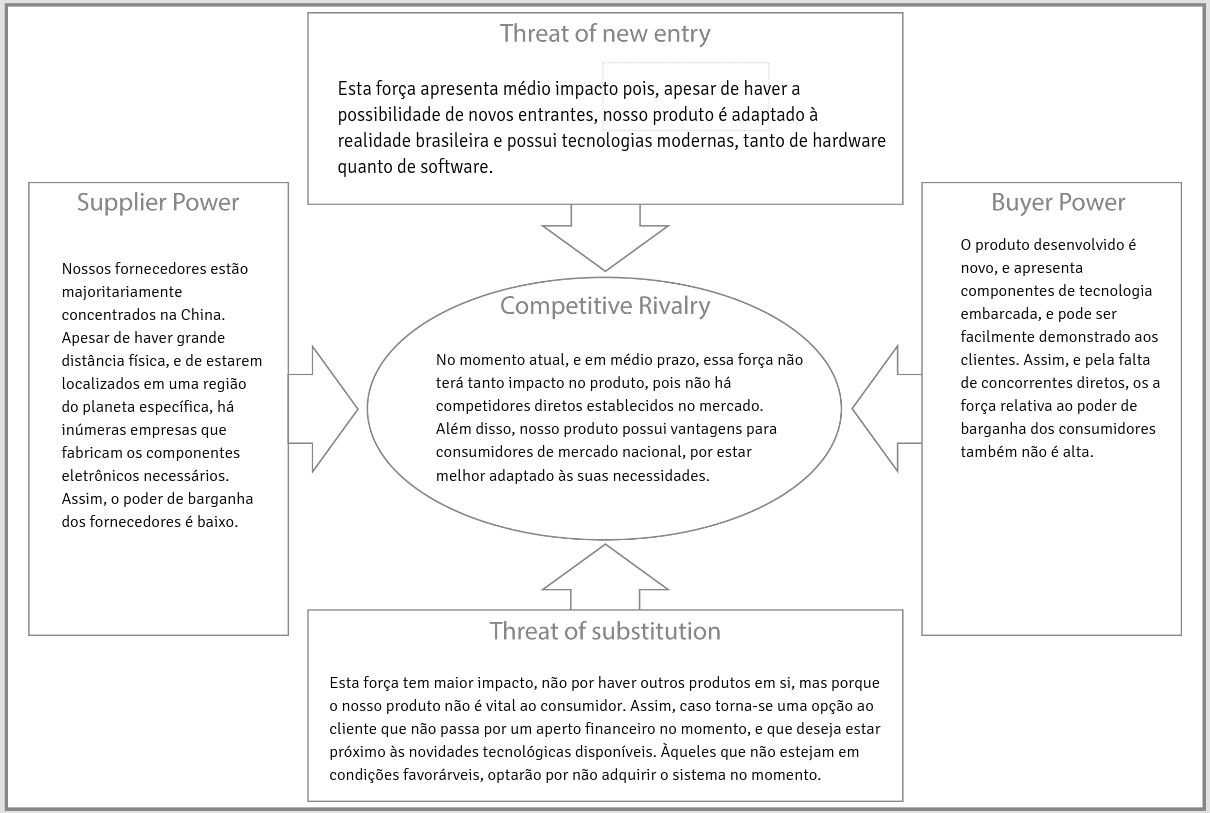
\includegraphics[width=0.8\textwidth]{porter}
	\end{center}
	\legend{Fonte: os autores}
\end{figure}

\subsection{Cadeia de Valor}

Conforme o definido por Michael Porter (Citar), para analisar todas as atividades desempenhadas pela empresa, com a finalidade de se criar vantagem competitiva em relação aos seus concorrentes, pode-se utilizar o modelo da Cadeia de Valor. Na \autoref{fig:cadeiaValor}, verifica-se a sua estrutura, que será detalhada em seguida.

\begin{figure}[H]
	\caption{\label{fig:cadeiaValor}Cadeia de Valor de Porter}
	\begin{center}
	    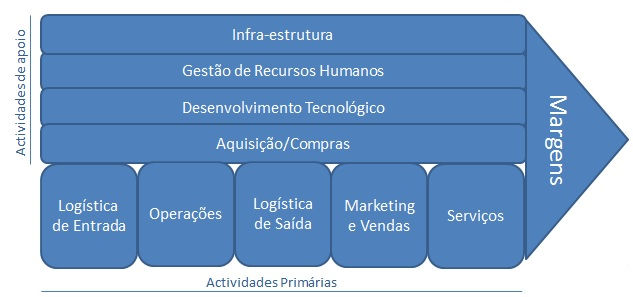
\includegraphics[scale=0.8]{cadeiaValor}
	\end{center}
	\legend{Fonte: CITAR http://www.gestaoporprocessos.com.br/o-modelo-de-cadeia-de-valor-de-michael-porter/}
\end{figure}

\begin{description}
    \item[Infraestrutura:]Todas as atividades necessárias para a empresa funcionar enquanto uma instituição. Emissões de relatórios, planejamentos, etc. fazem parte deste conjunto de atividades.

    \item[Gestão de Recursos Humanos:]Responsável pela manutenção dos funcionários, e a contratação de novos profissionais, bem como resolução de possíveis conflitos internos.

    \item[Desenvolvimento Tecnológico:]Essencial na Hedwig, já que faz parte da base de nossos produtos, e é um fator determinante para que a empresa esteja sempre na liderança do mercado.

    \item[Aquisição/Compras:]Negociação com os fornecedores e todas as atividades relativas a obtenção de matéria-prima.

    \item[Logística de Entrada:]A matéria prima é importada da China, e é transportada de navio até o porto de Santos, de onde seguirá para a empresa, por meio de uma empresa responsável pelo fretamento.

    \item[Operações:]Englobam as atividades de montagem física dos módulos, com a soldagem dos componentes nas placas de fenolite, e a instalação do microcontrolador.
    
    \item[Logística de Saída:]Utilização de serviços terceirizados para o transporte dos módulos às lojas.

    \item[Marketing e Vendas:]Atividades relacionadas com o oferecimento dos nossos produtos, tanto aos consumidores finais quanto a lojas específicas.

    \item[Serviço:]Atividades de pós-venda e suporte, para que o consumidor esteja sempre satisfeito com os nossos produtos, e quaisquer problemas encontrados devem ser resolvidos prontamente.
\end{description}

\section{Aspectos Éticos e de Segurança}

Por se tratar de um sistema presente dentro da casa de usuários, é de extrema importância que os dados que trafegam pelo mesmo sejam privados e que estejam armazenados de forma segura contra possíveis ações de \textit{hackers} e criminosos que tentem obtê-los, já que tratam-se de dados privados e sensitivos.

Para isso, serão utilizados apenas servidores de alta segurança para o armazenamento dos dados sensitivos.

Além disso, serão utilizados protocolos seguros, com criptografia, para todo o tráfego de dados do sistema.

\section{Comércio Eletrônico}

Haverá comércio inicialmente através de parceiros estratégicos em contato direto (revendedores locais, como instaladores de sistemas de alarmes), e comércio eletrônico após obtenção de escala, em duas etapas distintas:
\begin{enumerate}
	\item Email: canal consolidado de pedidos e comunicação com fornecedores e clientes (reclamações e pós compra);
	\item \textit{Site}: portal próprio, protegido por https com certificado digital, para a gestão de relacionamento com clientes e fornecedores, buscando expansão do \textit{e-commerce}. 
\end{enumerate}

\section{Social Business}

A publicidade será feita por página em redes sociais (Facebook), manutenção de página no GitHub, Canal no Youtube, Blog com tutoriais (e evolução do projeto). A ideia é fazer uma comunidade fiel ao conceito de casa conectada, através dos seguintes canais:
\begin{enumerate}
	\item \textbf{Facebook}: Usuários podem enviar feedbacks, requisições e espalhar anúncios de produtos prontos;
	\item \textbf{GitHub}: Usuários que gostam de programar podem interagir com o projeto (código livre);
	\item \textbf{Youtube}: Videos demonstrando funcionalidades e situações de uso, além de servir de suporte para o blog;
	\item \textbf{Blog}: Contém os vários tutoriais relativos aos diferentes usos dos módulos, além de notícias sobre a evolução do projeto (novas funcionalidades e módulos).
\end{enumerate}

\section{Inteligência de Negócios e Gestão de Riscos}

A inteligência de negócios se faz extremamente necessária no decorrer do desenvolvimento da empresa. A partir da mesma, será possível analisar quais estratégias estão sendo bem sucedidas e aceitas pelos usuários, e quais podem ser modificadas.

Para poder tomar decisões acertadamente, é de suma importância a coleta de dados nos quais possamos nos basear para analisar o negócio. Isso ocorrerá por meio de coleta de dados de uso, e coleta de acertos de previsões de aprendizado de máquina, para que possamos entender quão bem o produto está servindo às necessidades dos usuários.

A inteligência de negócios também será utilizada para ajudar a prever picos de demanda, para que a empresa esteja mais bem preparada para atender à mesma.

Segue matriz SWOT para análise de riscos:

\begin{figure}[htb]
	\caption{\label{fig:SWOT}Matriz SWOT}
	\begin{center}
		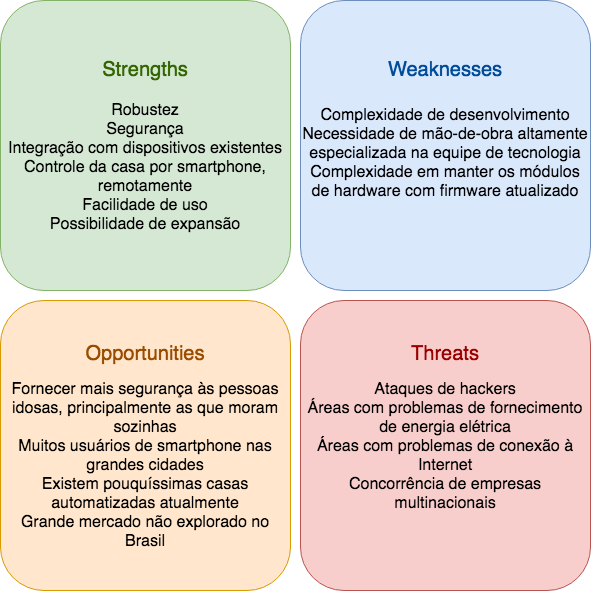
\includegraphics[scale=0.5]{SWOT}
	\end{center}
	\legend{Fonte: os autores}
\end{figure}
\chapter{Conclusões}

O estudo aqui apresentado foi extremamente relevante para o desenvolvimento do Projeto de Conclusão de Curso, nessa etapa final, por nos permitir ter uma visão completa de como o mesmo poderia funcionar como produto de uma empresa real.

Levar em consideração todos os aspectos de sistemas de informação permite explorar e refletir mais a fundo sobre cada aspecto do produto.

\end{document}
